

% \tikzset{every picture/.style={line width=0.75pt}} %set default line width to 0.75pt        

% \begin{tikzpicture}[x=0.75pt,y=0.75pt,yscale=-1,xscale=1]
% %uncomment if require: \path (0,300); %set diagram left start at 0, and has height of 300

% %Shape: Rectangle [id:dp8194440686845581] 
% \draw  [fill={rgb, 255:red, 223; green, 247; blue, 233 }  ,fill opacity=1 ] (177,190.34) -- (269.44,190.34) -- (269.44,246.4) -- (177,246.4) -- cycle ;
% %Shape: Rectangle [id:dp04310487861766332] 
% \draw  [color={rgb, 255:red, 0; green, 0; blue, 0 }  ,draw opacity=1 ][fill={rgb, 255:red, 223; green, 247; blue, 233 }  ,fill opacity=1 ] (269.44,53) -- (361.88,53) -- (361.88,109.06) -- (269.44,109.06) -- cycle ;
% %Shape: Rectangle [id:dp32975298478620196] 
% \draw  [fill={rgb, 255:red, 223; green, 247; blue, 233 }  ,fill opacity=1 ] (360.56,190.34) -- (453,190.34) -- (453,246.4) -- (360.56,246.4) -- cycle ;
% %Straight Lines [id:da23895133806094215] 
% \draw    (204.6,176.07) -- (253.73,109.22) ;
% \draw [shift={(254.91,107.61)}, rotate = 126.32] [color={rgb, 255:red, 0; green, 0; blue, 0 }  ][line width=0.75]    (10.93,-3.29) .. controls (6.95,-1.4) and (3.31,-0.3) .. (0,0) .. controls (3.31,0.3) and (6.95,1.4) .. (10.93,3.29)   ;
% \draw [shift={(203.41,177.68)}, rotate = 306.32] [color={rgb, 255:red, 0; green, 0; blue, 0 }  ][line width=0.75]    (10.93,-3.29) .. controls (6.95,-1.4) and (3.31,-0.3) .. (0,0) .. controls (3.31,0.3) and (6.95,1.4) .. (10.93,3.29)   ;
% %Straight Lines [id:da6917940815863461] 
% \draw    (379.05,111.28) -- (437.15,176.96) ;
% \draw [shift={(438.47,178.45)}, rotate = 228.5] [color={rgb, 255:red, 0; green, 0; blue, 0 }  ][line width=0.75]    (10.93,-3.29) .. controls (6.95,-1.4) and (3.31,-0.3) .. (0,0) .. controls (3.31,0.3) and (6.95,1.4) .. (10.93,3.29)   ;
% \draw [shift={(377.73,109.78)}, rotate = 48.5] [color={rgb, 255:red, 0; green, 0; blue, 0 }  ][line width=0.75]    (10.93,-3.29) .. controls (6.95,-1.4) and (3.31,-0.3) .. (0,0) .. controls (3.31,0.3) and (6.95,1.4) .. (10.93,3.29)   ;
% %Straight Lines [id:da8377933043589034] 
% \draw    (283.33,225.8) -- (349.32,225.8) ;
% \draw [shift={(351.32,225.8)}, rotate = 180] [color={rgb, 255:red, 0; green, 0; blue, 0 }  ][line width=0.75]    (10.93,-3.29) .. controls (6.95,-1.4) and (3.31,-0.3) .. (0,0) .. controls (3.31,0.3) and (6.95,1.4) .. (10.93,3.29)   ;
% \draw [shift={(281.33,225.8)}, rotate = 0] [color={rgb, 255:red, 0; green, 0; blue, 0 }  ][line width=0.75]    (10.93,-3.29) .. controls (6.95,-1.4) and (3.31,-0.3) .. (0,0) .. controls (3.31,0.3) and (6.95,1.4) .. (10.93,3.29)   ;

% % Text Node
% \draw (202.06,207.97) node [anchor=north west][inner sep=0.75pt]   [align=left] {{\fontfamily{pcr}\selectfont \textbf{Alice}}};
% % Text Node
% \draw (285.98,70.43) node [anchor=north west][inner sep=0.75pt]   [align=left] {\textbf{{\fontfamily{pcr}\selectfont Charlie}}};
% % Text Node
% \draw (393.58,208.77) node [anchor=north west][inner sep=0.75pt]   [align=left] {\textbf{{\fontfamily{pcr}\selectfont Bob}}};
% % Text Node
% \draw (285.14,138.91) node [anchor=north west][inner sep=0.75pt]  [font=\Large,color={rgb, 255:red, 255; green, 8; blue, 8 }  ,opacity=1 ]  {$\mathlarger{\mathlarger{\mathlarger{\mathlarger{\mathbf{\hat{\rho }_{abc}}}}}}$};


% \end{tikzpicture}



\tikzset{every picture/.style={line width=0.75pt}} %set default line width to 0.75pt        

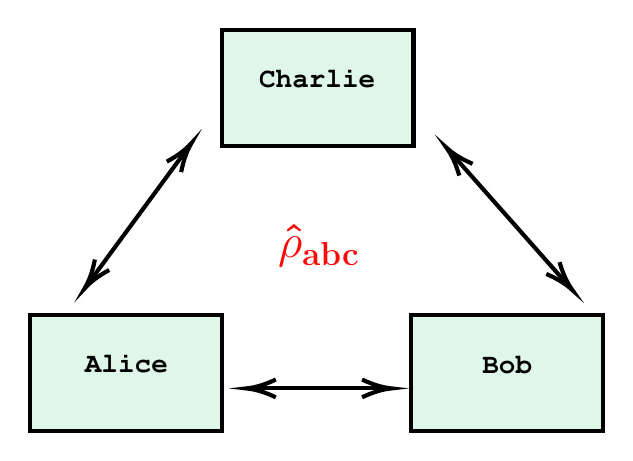
\begin{tikzpicture}[x=0.75pt,y=0.75pt,yscale=-1,xscale=1]
%uncomment if require: \path (0,300); %set diagram left start at 0, and has height of 300

%Shape: Rectangle [id:dp8194440686845581] 
\draw  [fill={rgb, 255:red, 223; green, 247; blue, 233 }  ,fill opacity=1 ][line width=1.5]  (177,190.34) -- (269.44,190.34) -- (269.44,246.4) -- (177,246.4) -- cycle ;
%Shape: Rectangle [id:dp04310487861766332] 
\draw  [color={rgb, 255:red, 0; green, 0; blue, 0 }  ,draw opacity=1 ][fill={rgb, 255:red, 223; green, 247; blue, 233 }  ,fill opacity=1 ][line width=1.5]  (269.44,53) -- (361.88,53) -- (361.88,109.06) -- (269.44,109.06) -- cycle ;
%Shape: Rectangle [id:dp32975298478620196] 
\draw  [fill={rgb, 255:red, 223; green, 247; blue, 233 }  ,fill opacity=1 ][line width=1.5]  (360.56,190.34) -- (453,190.34) -- (453,246.4) -- (360.56,246.4) -- cycle ;
%Straight Lines [id:da23895133806094215] 
\draw [line width=1.5]    (205.19,175.26) -- (253.14,110.03) ;
\draw [shift={(254.91,107.61)}, rotate = 126.32] [color={rgb, 255:red, 0; green, 0; blue, 0 }  ][line width=1.5]    (14.21,-4.28) .. controls (9.04,-1.82) and (4.3,-0.39) .. (0,0) .. controls (4.3,0.39) and (9.04,1.82) .. (14.21,4.28)   ;
\draw [shift={(203.41,177.68)}, rotate = 306.32] [color={rgb, 255:red, 0; green, 0; blue, 0 }  ][line width=1.5]    (14.21,-4.28) .. controls (9.04,-1.82) and (4.3,-0.39) .. (0,0) .. controls (4.3,0.39) and (9.04,1.82) .. (14.21,4.28)   ;
%Straight Lines [id:da6917940815863461] 
\draw [line width=1.5]    (379.71,112.03) -- (436.49,176.21) ;
\draw [shift={(438.47,178.45)}, rotate = 228.5] [color={rgb, 255:red, 0; green, 0; blue, 0 }  ][line width=1.5]    (14.21,-4.28) .. controls (9.04,-1.82) and (4.3,-0.39) .. (0,0) .. controls (4.3,0.39) and (9.04,1.82) .. (14.21,4.28)   ;
\draw [shift={(377.73,109.78)}, rotate = 48.5] [color={rgb, 255:red, 0; green, 0; blue, 0 }  ][line width=1.5]    (14.21,-4.28) .. controls (9.04,-1.82) and (4.3,-0.39) .. (0,0) .. controls (4.3,0.39) and (9.04,1.82) .. (14.21,4.28)   ;
%Straight Lines [id:da8377933043589034] 
\draw [line width=1.5]    (284.33,225.8) -- (348.32,225.8) ;
\draw [shift={(351.32,225.8)}, rotate = 180] [color={rgb, 255:red, 0; green, 0; blue, 0 }  ][line width=1.5]    (14.21,-4.28) .. controls (9.04,-1.82) and (4.3,-0.39) .. (0,0) .. controls (4.3,0.39) and (9.04,1.82) .. (14.21,4.28)   ;
\draw [shift={(281.33,225.8)}, rotate = 0] [color={rgb, 255:red, 0; green, 0; blue, 0 }  ][line width=1.5]    (14.21,-4.28) .. controls (9.04,-1.82) and (4.3,-0.39) .. (0,0) .. controls (4.3,0.39) and (9.04,1.82) .. (14.21,4.28)   ;

% Text Node
\draw (202.06,207.97) node [anchor=north west][inner sep=0.75pt]   [align=left] {{\fontfamily{pcr}\selectfont \textbf{Alice}}};
% Text Node
\draw (285.98,70.43) node [anchor=north west][inner sep=0.75pt]   [align=left] {\textbf{{\fontfamily{pcr}\selectfont Charlie}}};
% Text Node
\draw (393.58,208.77) node [anchor=north west][inner sep=0.75pt]   [align=left] {\textbf{{\fontfamily{pcr}\selectfont Bob}}};
% Text Node
\draw (316.39,157.15) node  [font=\LARGE,color={rgb, 255:red, 255; green, 8; blue, 8 }  ,opacity=1 ]  {$\mathlarger{\mathlarger{\mathlarger{\mathlarger{\mathbf{\hat{\rho }_{abc}}}}}}$};


\end{tikzpicture}
